
\begin{figure}

\begin{minipage}{0.5\textwidth}
\small
\begin{verbatim}
function visit( Node v ) {
  globals.time++;
  discovery[ v.getId() ] = globals.time;
  beginStep();
  v.setLabel( "" + discovery[ v.getId() ] );
  v.selected( true );
  endStep();
  for_outgoing( v, e, w ) {
    beginStep();
    if ( ! w.isSelected() ) {
      e.setSelected(true);
       visit( w );
    }
    else if ( finish[ w.getId() ] == 0 ) {
      e.setLabel( "B" );  /* ancestor */
    }
    else if ( finish[ w.getId() ]
              > discovery[ v.getId() ] ) {
      e.setLabel( "F" );  /* descendant */
    }
    else {
      e.setLabel( "C" );
    }
    endStep();
  }
  beginStep();
  globals.time++;
  finish[ v.getId() ] = globals.time;
  v.mark();
  v.setLabel( "" + discovery[ v.getId() ]
              + "/" + finish[ v.getId() ] );
  endStep();
}

setDirected( true );

beginStep();
for_nodes( u ) {
    u.setLabel("");
}
for_edges( e ) {
    e.setLabel("");
}
endStep();

for_nodes( u ) {
    if ( ! u.isSelected() ) {
        visit( u, null );
    }
}

\end{verbatim}
\end{minipage}
\begin{minipage}{0.49\textwidth}
\centering

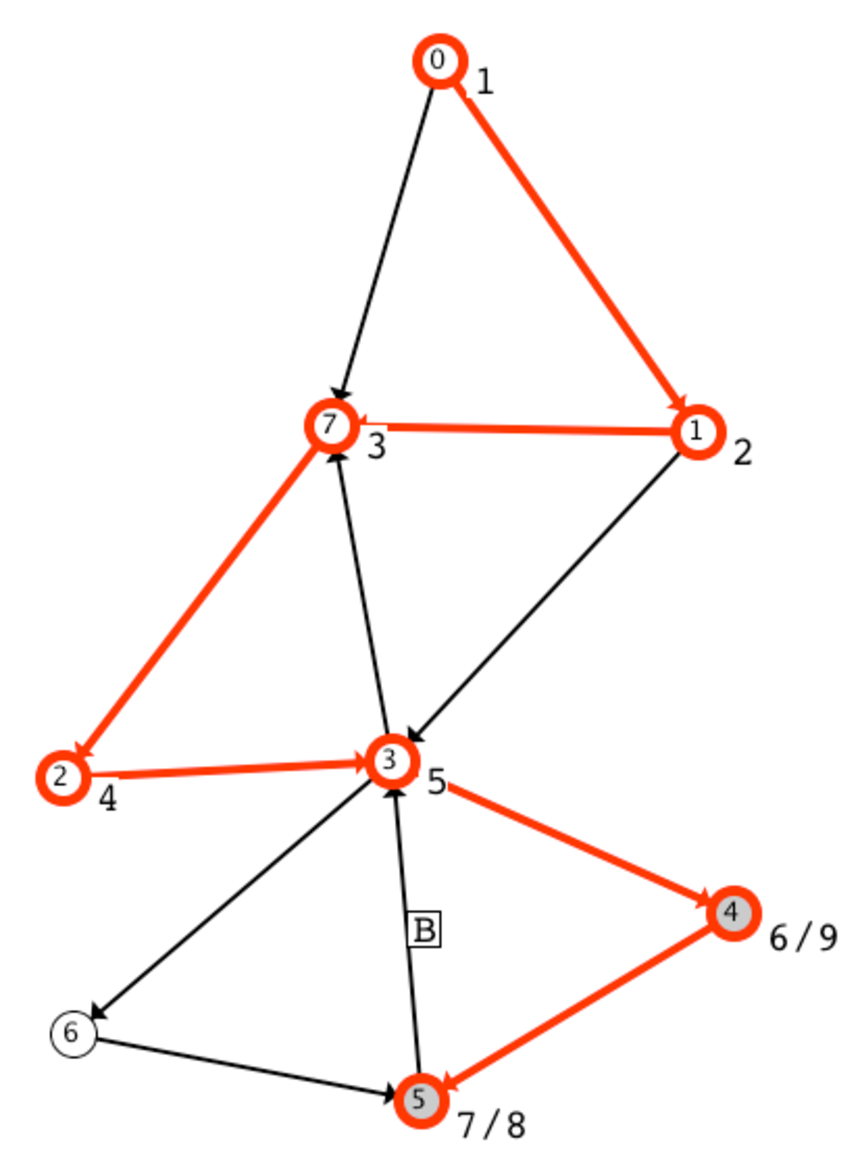
\includegraphics[scale=0.5]{X_dfs_d_1}

After first non-tree edge is labeled. 

\medskip

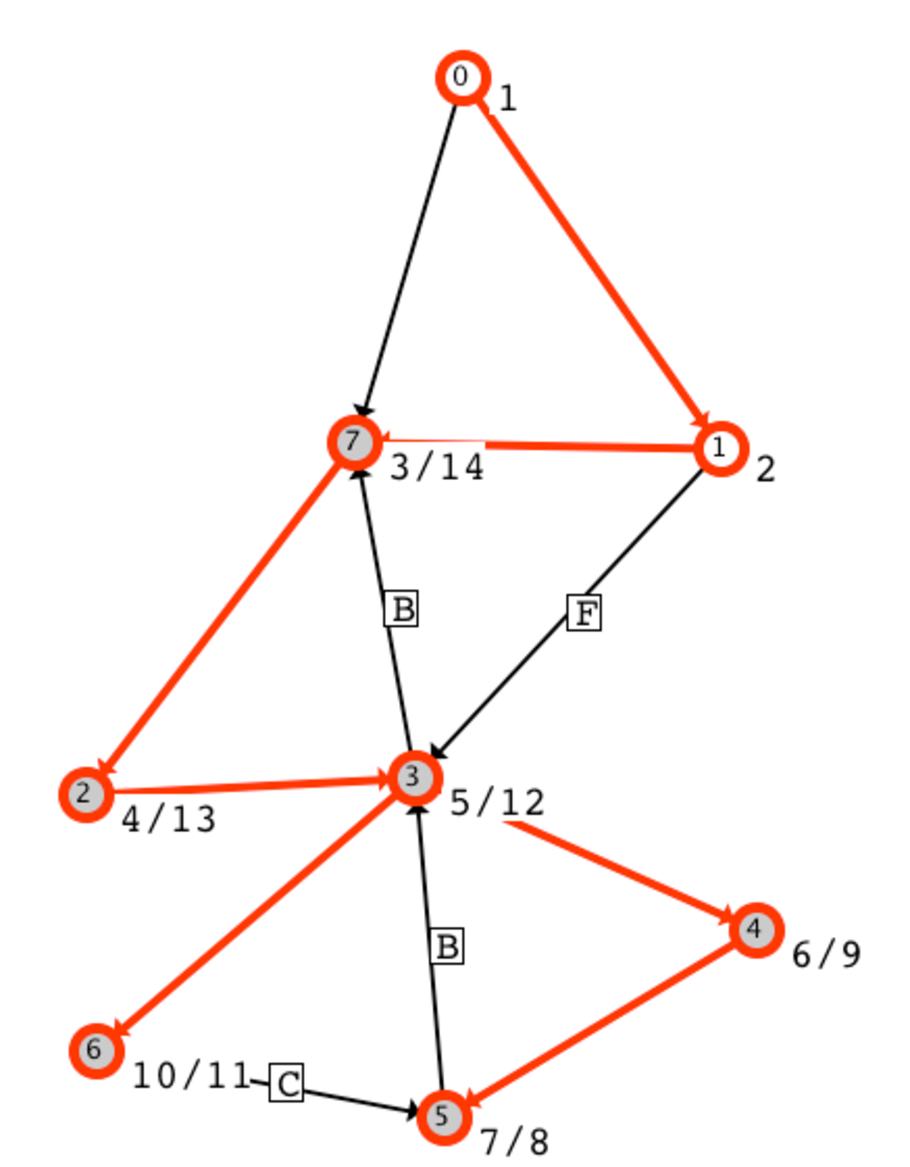
\includegraphics[scale=0.5]{X_dfs_d_2}

After all but one non-tree edges have been labeled.

\end{minipage}
\caption{Implementation of a depth-first search animation
  with an illustration of the graph panel during execution.}
\label{fig:dfs}
\end{figure}


Fig.~\ref{fig:dfs} illustrates an animation of depth-first search.
The code and definitions follow those of Cormen et al.~\cite{2009-Intro_to_Algorithms-Cormen}.
Tree edges are highlighted (selected)
and non-tree edges are labeled as \textbf{B}ack edges,
\textbf{F}orward edges or \textbf{C}ross edges.
White nodes, not yet visited,
are neither highlighted (selected) nor marked;
Gray nodes, visited but the visit is not finished, are highlighted only;
and black nodes, visit is completed, are both highlighted and 
marked.
Labels on nodes indicate the discovery and finish times, separated by a slash.

The \verb+setDirected(true)+ statement
ensures that the graph is displayed and treated as a directed graph.
For depth-first search, unlike Dijkstra's algorithm, we need to write a different algorithm/animation to deal with the special case that arises because tree
edges are also back edges when regarded as bidirectional.

As with Kruskal's algorithm, the handling of global variables is awkward.
But here, the global variable \verb+time+ cannot be declared \verb+final+
since that would prevent any changes to its value. The workaround, not shown
in the figure due to space constraints, is:

\begin{verbatim}
class GlobalVariables {
    public int time;
}
final GlobalVariables globals = new GlobalVariables();
\end{verbatim}

This is yet another case where some macro preprocessing could make global
variables mare transparent. A useful construct might be along the lines of
\begin{verbatim}
globals {
    int time;
    // and, using the syntax suggested in the discussion of Kruskal's algorithm
    int discovery[ Node ];
    int finish[ Node ];
}
\end{verbatim}
And then the preprocessor could do the necessary conversion, making, among
other things, the use of simply \verb+time+ instead of \verb+globals.time+
possible.



